\documentclass{article}
\usepackage{graphicx}
\graphicspath{ {./} }
\usepackage{color}

\usepackage{amsmath}
\usepackage{commath}
\usepackage{amssymb}
\usepackage{listings}
\usepackage{algorithm2e}
\usepackage{float}

\usepackage{hyperref}
\hypersetup{linktoc=all}

\usepackage{listings}
\usepackage{geometry}
\geometry{margin=1in}
\usepackage{color}
\definecolor{light-gray}{gray}{0.95}
\lstset{numbers=right, 
                numberstyle=\tiny, 
                breaklines=true,
                backgroundcolor=\color{light-gray},
                numbersep=5pt,
                xleftmargin=.5in,
                xrightmargin=.5in} 

\sloppy
\definecolor{lightgray}{gray}{0.5}
\setlength{\parindent}{0pt}

\begin{document}

\title{Lab 3: Simple Steganography}
\author{Brian Hosler \& Sarah Peachey }
\maketitle 

    

\subsection*{Part 1}

\begin{par}
extract the metadata tag associated with image   1) reading the quatization tables used to encode and decode in the   jpeg header   2) compare to list of digital camera models Need wine to use JPEGsnoop.exe :(
\end{par} \vspace{1em}


\subsection*{Part 2}

\qquad JPEG compression can be detected by identifying $8 \ \times \ 8$
grids across the image. One way to quantify the blocking is to make the same
calculation at the center of an $8 \ \times \ 8$ block and at the edge of an
$8 \ \times \ 8$ block and compare the error. If there are no blocking
artifacts then the error should be small, if there are blocking artifacts
the values at the corners will greatly varry from the center of the block. 

\includegraphics [width=4in]{block}

Using the $[A, B, C, D, E, F, G, H]$, noted above the \eqref{eq1} and
\eqref{eq2} are calculated
for every $8 \ \times \ 8$ block in the image. 

\begin{align}
	Z'(i,j)=\abs{A-B-C+D}\label{eq1}\\
	Z''(i,j)=\abs{E-F-G+H}\label{eq2}
\end{align}

The values are then put into a normalized histogram, if the center values,
Z', histogram looks the same as the edge values Z\'', histogram; then
the image was jpeg compressed. 

\begin{verbatim}
im1=imread('Assignment4Files/blockArtifacts1.tif');
k1=blockDetect(im1)

im2=imread('Assignment4Files/blockArtifacts2.tif');
k1=blockDetect(im2)

im3=imread('Assignment4Files/blockArtifacts3.tif');
k1=blockDetect(im2)

type('blockDetect.m')
\end{verbatim}

        \color{lightgray} \begin{verbatim}The strength of the blocking fingerprint is 1.498818e+00.
So the image was JPEG compressed 

k1 =

    1.4988

The strength of the blocking fingerprint is 1.496792e+00.
So the image was JPEG compressed 

k1 =

    1.4968

The strength of the blocking fingerprint is 1.496792e+00.
So the image was JPEG compressed 

k1 =

    1.4968


function [ k ] = blockDetect( im )
%blockDetect implements the Fan and de Quieroz?s JPEG blocking artifact
    % detecting algorithm. inputs any image and output the k, blcoking 
    % strength value. 
    Zp=[]; 
    Zpp=[];
    [r,c]=size(im); 
    for i=1:8:r-8 % dont do the last 8x8 block in row or cols 
        for j=1:8:c-8
            grid=im(i:i+7,j:j+7); % grid plus one 
            A=grid(4,4); 
            B=grid(4,5); 
            C=grid(5,4); 
            D=grid(5,5); 
            Zp=[Zp, double(abs(A-B-C+D))]; 
            E=grid(8,8); 
            F=im(i+7,i+8); 
            G=im(i+8,i+7); 
            H=im(i+8,i+8); 
            Zpp=[Zpp, double(abs(E-F-G+H))]; 
        end 
    end 
    % 2)
    figure 
    HI=histogram(Zp,255); 
    HI.Normalization = 'probability'; 
    hold on 
    HII=histogram(Zpp,255); 
    HII.Normalization = 'probability'; 
    legend('Normalized center values','Normalized edge values')
    % 3)
    k=sum(abs(HI.Values-HII.Values)); 
    n=0.25; 
    % 4) 
    jpegDetect = (k>n); 
    fprintf('The strength of the blocking fingerprint is %d.\n',k); 
    if jpegDetect==1
        fprintf('So the image was JPEG compressed \n')
    else
        fprintf('So the image was not JPEG compressed \n')
    end

end

\end{verbatim} \color{black}
    
As seen below the Z' and Z\'', histograms look very different. Also
the error of the two histograms was taken, called the blocking fingerprint.
The blocking fingerprint was then compared to a threshold of
0.25 to see if jpeg compression was detected. 

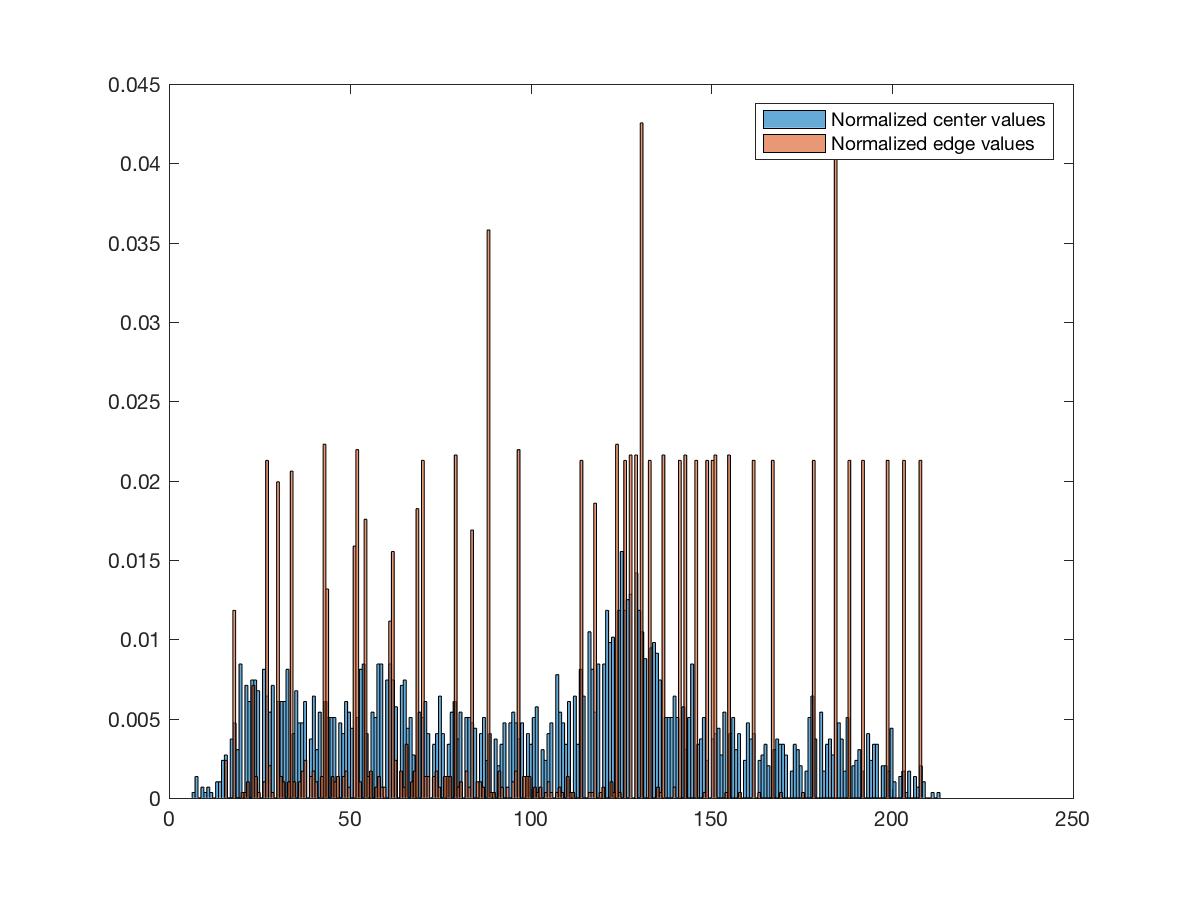
\includegraphics [width=4in]{lab4_01.eps}

\includegraphics [width=4in]{lab4_02.eps}

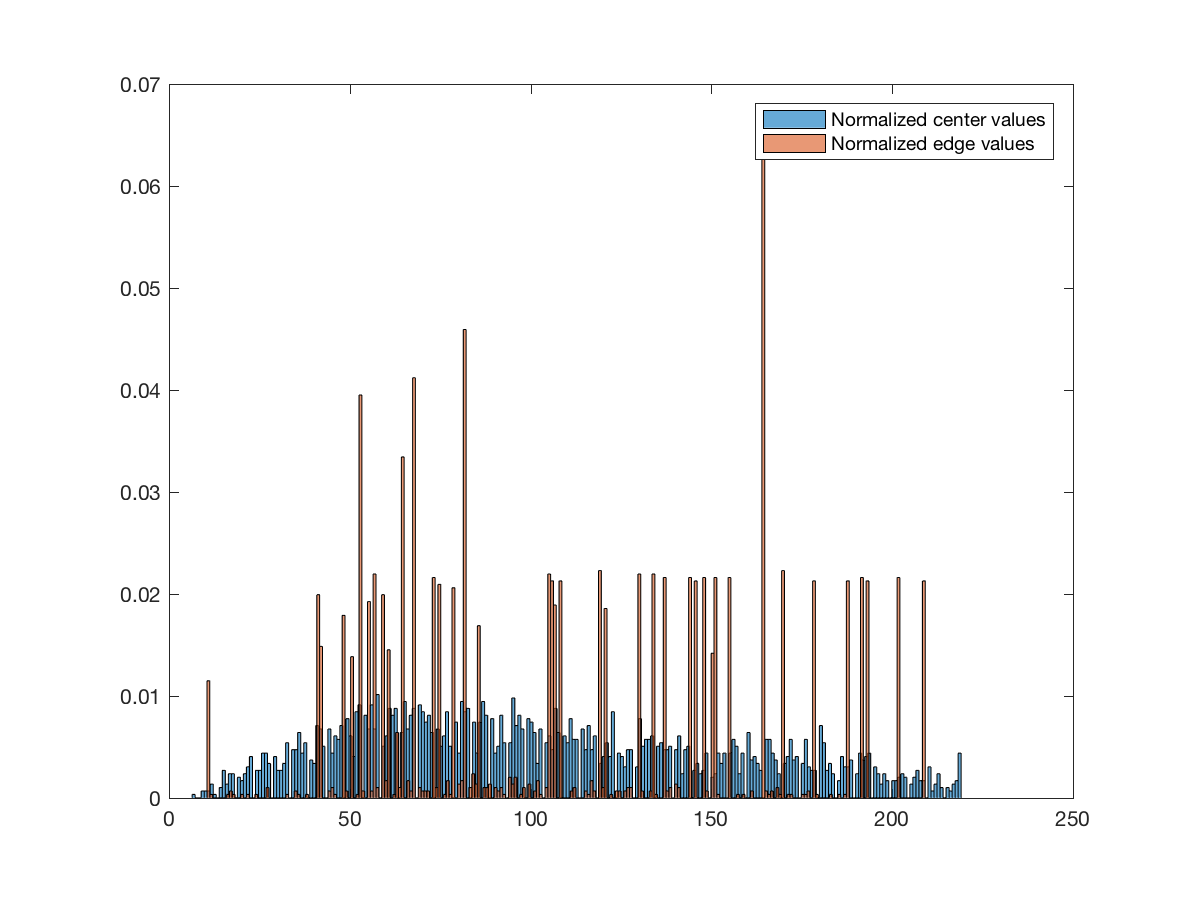
\includegraphics [width=4in]{lab4_03.eps}



\end{document}
    
